\chapter{Application}
Nous avons vu dans le chapitre 1 de ce mémoire que l'utilisation d'algorithmes de type boites noires dans l'aide à la prise de décision soulevait des questions, notamment sur l'éthique, la fiabilité et la performance. Dans cette partie, nous allons mettre en application nos recherches présentées dans l'état de l'art afin de déterminer si l'interprétabilité d'un modèle boîte noire nous permettrai de résoudre ces problèmes.
\section{Mise en évidence de biais}
L'objectif de cette partie est de démontrer que rendre un modèle boite noire interprétable permettrai de mettre en évidence des biais discriminatoire. Pour cela, nous allons créer un modèle prédictif à partir d'un jeu de données comportant possiblement des biais, puis d'utiliser l'outil SHAP afin d'essayer de mettre en évidence les éventuels biais présents dans notre jeu de données. Le code de cette section est disponible sur mon GitHub \cite{shapMyDepot} et suit, entre autre, le tutoriel de "Towards Data Science"\cite{shapTuto}
\subsection{Le jeu de données}
Afin de savoir si utiliser une méthode de compréhension de boites noires aurai permis de mettre en évidence les biais présents dans l'intelligence artificielle dite sexiste de l'entreprise Amazon (évoquée dans l'introduction de ce mémoire), nous appliquerons ces méthodes sur un exemple similaire. Pour rappel, cette IA rejetait les CVs de femmes car elle avait été entraînée en se basant sur les personnes employées par l'entreprise dans le passé et que ces personnes étaient majoritairement des hommes, l'IA a donc conclue qu'il était préférable d'embaucher un homme plutôt qu'une femme.\par
Pour cette expérimentation, nous allons utiliser un jeu de données qui nous donne des informations sur des étudiants ainsi que leurs notes à différents examens. Les données d'entrée de notre modèle seront donc de type tabulaire. Ce jeu de données disponible ici \cite{examScore} ressemble à cela (Figure \ref{studentsPerformanceDataSet}) :

\begin{figure}[h]
    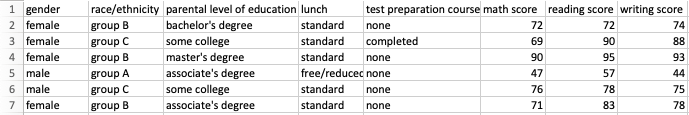
\includegraphics[scale=0.65]{src_img/studentsPerformanceDataSet.png}
    \caption{Jeu de donnée des performances des étudiants}
    \label{studentsPerformanceDataSet}
\end{figure}

À noter, que ce jeu de données est fictif et généré aléatoirement. Notre but est de créer un modèle qui prédira la moyenne d’un étudiant en fonction de son sexe, de son ethnie, du niveau d’éducation de ses parents, de son régime alimentaire et de sa préparation aux tests. Pour ce faire, le jeu de données a été modifié en retirant les trois colonnes de scores afin d'en créer qu'une seule correspondant à la moyenne des trois. Nous obtenons donc le résultat présenté dans la figure \ref{studentsPerformanceDataSetModif} : 
\begin{figure}[h]
    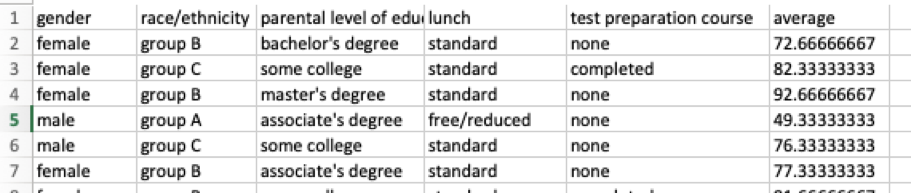
\includegraphics[scale=1]{src_img/StudentsPerformanceDataSetModif.png}
    \caption{Jeu de donnée final}
    \label{studentsPerformanceDataSetModif}
\end{figure}
Une fois notre modèle entraîné à prédire la moyenne potentielle d'un étudiant à partir de ces caractéristiques, on pourrai imaginer l'utiliser pour le recrutement universitaire. Mais (en dépit du fait que ces caractéristiques ne sont pas très pertinentes) notre modèle de recrutement est-il réellement fiable ? Pourrait-il être discriminant pour certaines ethnies ou pour un certain sexe ? Nous allons essayer de le découvrir en comprenant comment les caractéristiques d'entrée influent sur notre prédiction.

\subsection{Création du modèle prédictif}
La première étape sera donc de créer un modèle prédictif et de l'entraîner sur notre jeu de données. Pour ce faire, nous allons utilisé l'algorithme des forêts d'arbres décisionnels (random forest) qui fait partie de la famille des ensembles d'arbres vu dans l'état de l'art partie 2.2.3. Cet algorithme reposant sur l'apprentissage par arbre de décision consiste à effectuer un apprentissage en parallèle sur de multiples arbres de décision construits aléatoirement et entraînés sur des sous-ensembles de données différentes selon le principe du bagging. Le baggin consiste à réduire la variance d'un arbre de décision afin de palier à son instabilité. Les prédictions de tous ces arbres sont ensuite moyennées afin de nous donner un résultat.\par
Afin de créer notre modèle, nous allons utiliser une bibliothèque Python destinée à l'apprentissage automatique appelée Scikit-learn (sklearn)\cite{sklearnDepot}. Cette bibliothèque a été initiée en 2007 par David Cournapeau en tant que projet Google Summer of Code qui est un programme organisé par l'entreprise Google où des étudiants travaillent pendant l'été sur un projet pour lequel l'étudiant a postulé. Open source et comptant de nombreux collaborateurs, cette bibliothèque mettant à notre disposition une multitude d'outils pour le machine learning est devenue la référence dans son domaine notamment grâce à sa complétude et sa simplicité d'utilisation.\par
Avec Scikit-learn, la création de forêts d'arbres décisionnels se fait à l'aide d'une classe appelée \textit{RandomForestRegressor}, mais avant de l'utiliser nos données doivent être adaptées afin d'y être compatible. Dans un premier temps, il nécessaire d'enlever la colonne "average" car ce ne sera pas une caractéristique d'entrée mais la valeur à prédire (target). De plus, la fonction de forêts d'arbres décisionnels ne peux pas prendre en données d'entrée un tableau contenant des valeurs qualitatives (non-numérique). Afin d'être adapté à notre modèle, notre jeu de données a donc dû être encodé en créant une colonne par variables dans le but de n'avoir que des entrées numériques, par exemple la colonne "gender" devient deux colonnes "female" et "male" prenant 0 ou 1 comme valeur. Cette transformation des données est appelée "encodage one-hot" ou "encodage 1 parmi n". Pour ce faire, Scikit-learn met à notre disposition une classe : \textit{"from sklearn.preprocessing import OneHotEncoder"} nous permettant de procéder simplement à cet encodage. Ainsi, pour notre jeu de données, nous passons de cinq colonnes d'entrée à dix-sept colonnes qui sont : \medbreak
['x0\_female' 'x0\_male' 'x1\_group A' 'x1\_group B' 'x1\_group C' 'x1\_group D' 'x1\_group E' "x2\_associate's degree" "x2\_bachelor's degree" 'x2\_high school' "x2\_master's degree" 'x2\_some college' 'x2\_some high school' 'x3\_free/reduced' 'x3\_standard' 'x4\_completed' 'x4\_none']\medbreak
Où "x0" correspond à la transformation de la première colonne, "x1" à la transformation de la deuxième colonne et ainsi de suite.\par
Maintenant que nos données sont prêtes, nous allons créer notre modèle à l'aide de la classe \textit{RandomForestRegressor}. Pour ce faire, il nous suffit de l'initialiser en choisissant, pour notre cas, : la profondeur maximale des arbres (six dans notre cas), le nombre d'arbres dans la forêt (dix dans notre cas). Puis de l'entraîner à l'aide de la fonction \textit{"fit"} prenant en argument les caractéristiques d'entrées et la colonne que l'on souhaite prédire (average dans notre cas).

\subsection{Explication de notre prédiction}
Notre modèle étant prêt, nous allons pouvoir nous demander s'il n'a pas été biaisé involontairement par notre jeu de données. Pour ce faire, nous allons utiliser l'outil d'interprétation Python SHAP vu dans notre état de l'art. La première chose à faire est de déterminer la valeur de Shapley de notre modèle. Pour ce faire, la librairie SHAP met à notre disposition une fonction prenant en paramètre notre modèle ainsi que nos données d'entraînement. Comme décrit dans l'état de l'art partie 2.3.2, cette fonction va sonder notre modèle de multiple fois en faisant varier les données d'entrées afin de déterminer l'impact de ces données sur notre prédiction.\par
Une fois notre valeur de Shapley obtenue, nous pouvons afficher différent graphique afin de mieux comprendre les raisons de nos prédictions. La figure \ref{shapPlotBar} est un graphique généré par la fonction \textit{"summary\_plot avec pour type "bar""} de SHAP fournissant une explication globale de notre modèle de type importance des variables (features importance). L’importance des variables est calculée en moyennant la valeur absolue des valeurs de Shapley de chaque variable pour chaque exemple de notre jeu de données.

\begin{figure}[h]
    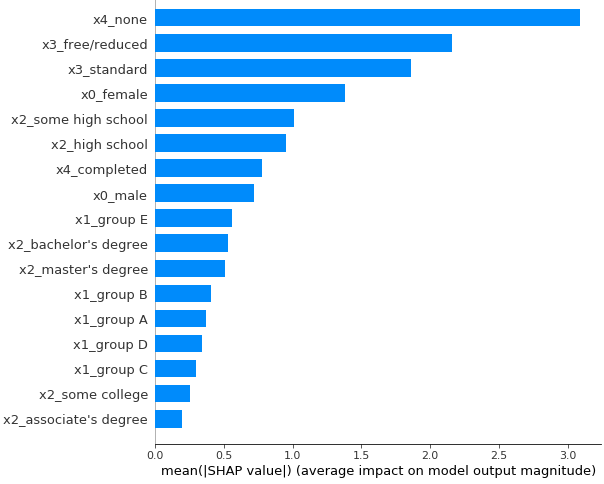
\includegraphics[scale=0.6]{src_img/shapPlotBar.png}
    \caption{Importance des variables d'entrées dans notre prédiction}
    \label{shapPlotBar}
\end{figure}

On voit donc sur notre graphique que la non-préparation aux tests et qu'un régime alimentaire équilibré sont les deux entrées aillent le plus d'impact sur notre prédiction, mais nous ne sommes pour le moment pas en mesure de savoir si cet impact est positif ou négatif.


Afin d'entrer plus dans le détail, SHAP nous offre d'autres graphiques comme par exemple la figure \ref{shapPlotDetail} toujours généré avec la fonction \textit{"summary\_plot"}. Sur ce graphique, chaque point représente une valeur de Shapley pour la variable pour chacune des instances. Les points rouges représentent un impact positif sur notre prédiction et les points bleu représentent un impact négatif. Nos données d'entrée étant constituées de valeurs binaires, ce graphique se lis de cette manière : si la valeur est positive et que la couleur est bleu alors la variable a un impact négatif sur notre valeur de sortie et inversement pour la couleur rouge. Par exemple la non-préparation au test et un régime alimentaire équilibré ont une influence négative sur notre moyenne. On peut aussi voir qu'être une femme a un impact positif alors qu'être un homme a un impact négatif. L’ethnie de type D sera aussi favorisée. Ces résultats laissent penser qu'utiliser ce modèle pour le recrutement universitaire aura un effet discriminatoire pour les hommes qui seront défavorisés, ce qui ressemble à l’IA d’Amazon évoquée précédemment.
\begin{figure}[h]
    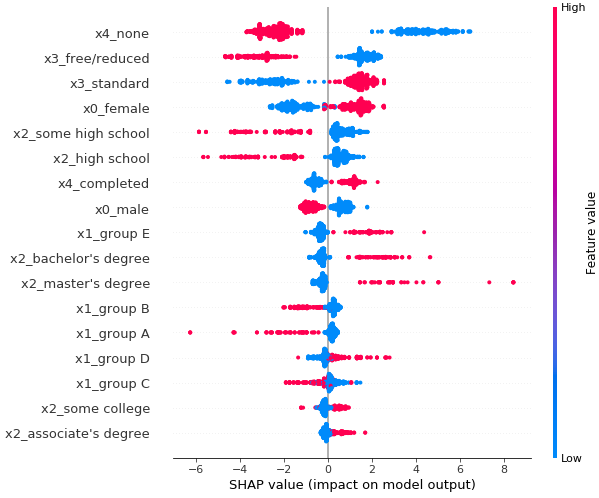
\includegraphics[scale=0.6]{src_img/shapPlotDetail.png}
    \caption{Détail de l'explication de l'importance des variables}
    \label{shapPlotDetail}
\end{figure}
Il nous est aussi possible de fournir une interprétation local c'est-à-dire de voir pourquoi notre boite noire a donnée un tel résultat pour une instance précise. La figure \ref{shapPlotLocal}, généré avec la fonction \textit{"dependence\_plot"} de SHAP, nous montre un exemple d'interprétation local. On vois que pour cette instance notre modèle a estimé que l'étudiant aurai 60.62 de moyenne. Comme pour l'exemple précédent, les variables aillant un impact positif sont affichées en rouge et celles ayant un impact négatif sont affichées en bleu. On voit donc que pour cette instance l'entraînement à l'épreuve, le régime alimentaire et le sexe influence négativement notre moyenne alors que le niveau d’éducation des parents a une influence positive.
\begin{figure}[h]
    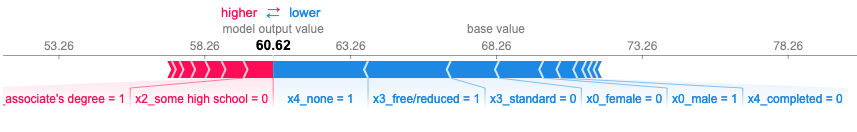
\includegraphics[scale=0.5]{src_img/shapPlotLocal.png}
    \caption{Explication de la prédiction pour une instance précise}
    \label{shapPlotLocal}
\end{figure}

\subsection{Bilan}
 Après l'inspection de notre modèle, nous avons pu voir qu'il jugeait les femmes plus performantes que les hommes et que son utilisation dans le recrutement universitaire aurai eut un impact discriminant sur les étudiants postulant. L'utilisation d'une méthode d'interprétabilité sur notre boite noire nous a donc permis de mettre en évidence un biais de discrimination présent dans notre jeu de donnée. Bien sûr, notre exemple étant trivial on aurai pu directement se rendre compte que les caractéristiques d'entrées n'étaient pas réellement pertinentes pour prédire la moyenne d'un étudiant.\par
 Nous pouvons donc dire que qu'il est important de vérifier la pertinence des entrées de notre modèle, aussi utiliser un algorithme permettant que comprendre la logique interne de notre boite noire est important afin d'éviter tous problèmes.

\section{Améliorer la fiabilité}
L'intelligence artificielle pose aussi des problèmes de fiabilités, notamment dans le domaine médical. Afin de savoir si rendre un modèle interprétable permettrai d'améliorer sa fiabilité et de vérifier s'il se base sur les bons éléments pour donner ses prédictions, nous allons appliquer l'algorithme LIME vu dans l'état de l'art à un modèle issu du monde médical.

\subsection{Le jeu de données}
Pour cette expérimentation, nous allons utiliser un jeu de données contenant des images de radiographies. Le but sera de créer un modèle permettant de détecter si le patient de la radiographie est atteint de pneumonie. Ce jeu de données disponible ici \cite{kagglePneumonia} est visible sur la Figure \ref{pneumoniaImg} :
\begin{figure}[h]
    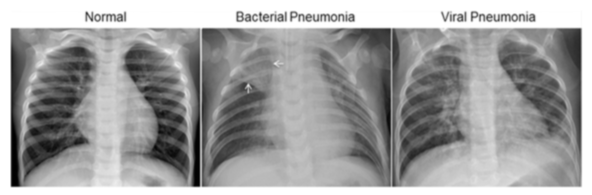
\includegraphics[scale=0.7]{src_img/pneumoniaImg.png}
    \caption{Exemple d'images présentes dans le jeu de donnée de pneumonie}
    \label{pneumoniaImg}
\end{figure}
Le jeu de données contient donc des radiographies de cages thoraciques saines ou malade. Dans la partie suivante, nous allons donc créer un modèle prenant en entrée une radiographie et nous donnant une prédiction sur l'état de santé du patient.

\subsection{Création du modèle prédictif}
Afin de prédire si la radiographie présente une pneumonie ou pas, nous allons créer un réseau de réseau de neurones à convolution (Convolutional Neural Networks). Cet algorithme, faisant partie de la famille des réseaux de neurones profond vu dans l'état de l'art parti 2.2.3, va ajouter des filtres et des couches à notre image d'entrée afin de pouvoir détecter plus de patterns sur notre image que le ferai un réseau de neurones classique. La figure \ref{CNNExplain} nous montre le fonctionnement d'une convolution, elle consiste en l'enchaînement de deux étapes : le "filtrage" et le "pooling" pour finir sur un réseau de neurones profond classique.
\begin{figure}[h]
    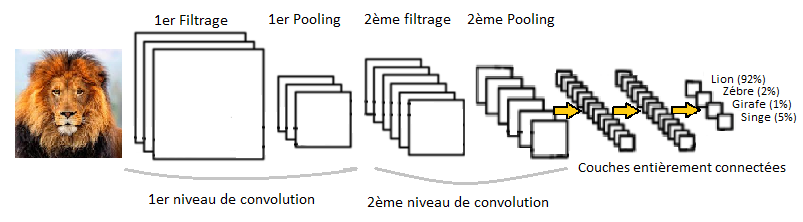
\includegraphics[scale=0.7]{src_img/CNNExplain.png}
    \caption{Schéma expliquant la convolution. \textit{Source : \cite{CnnExplainArticle}}}
    \label{CNNExplain}
\end{figure}

Le filtrage consiste à appliquer un filtre sur l'image afin de créer plusieurs images différentes à partir de l'image d'entrée, il permet de faire ressortir par exemple les contours, la couleur, la luminosité, etc... Ensuite, le pooling va prendre les images filtrées et vas les réduire en extrayant les valeurs importantes des pixels. Pour ce faire il va prendre, par exemple, un carré de trois pixel sur trois et le transformé en un seul pixel de la valeur du pixel le plus haut ou de la moyenne des pixels du carré. Afin d'y voir plus clair, la figure \ref{CNNpooling} nous schématise le fonctionnement du pooling. Ainsi, sur la figure, l'image qui faisait à l'origine neuf par neuf pixels en fait plus que sept par sept ce qui aura pour effet de diminuer les valeurs d'entrées et donc notre temps de calcul final.

\begin{figure}[h]
    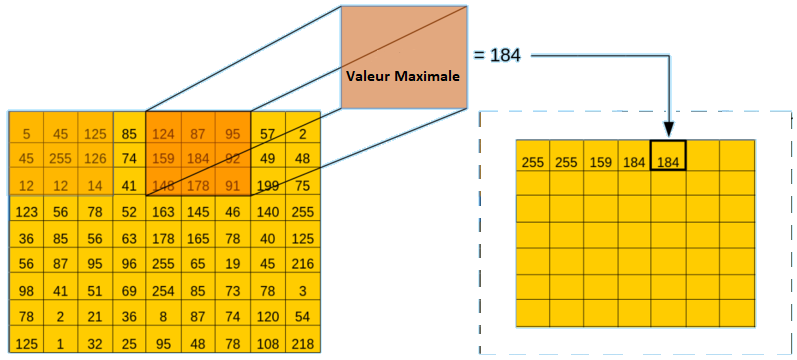
\includegraphics[scale=0.5]{src_img/CNNpooling.png}
    \caption{Explication d'un pooling de taille trois par trois. \textit{Source : \cite{CnnExplainArticle}}}
    \label{CNNpooling}
\end{figure}

Le code du modèle de cette application est disponible sur mon GitHub \cite{pneumoniaDepot} et a été créé en Python à l'aide de TensorFlow 2.0.\par
TensorFlow\cite{tensorflowDepot} est un outil d'apprentissage automatique initié par Google en 2011 devenu en 2015 open source et comptant de nombreux collaborateurs. TensorFlow met à notre disposition une API stable pour les langages Python et C++, et est devenu l'un des outils les plus utilisés en matière d'intelligence artificielle notamment pour la création d'architecture de réseau de neurones artificiels.\par
Tensorflow va donc nous permettre de créer notre réseau à convolution pour la détection de pneumonie dont l'architecture est présenté sur la figure \ref{CNNPneumoniaArchi}.\par
\begin{figure}[h]
    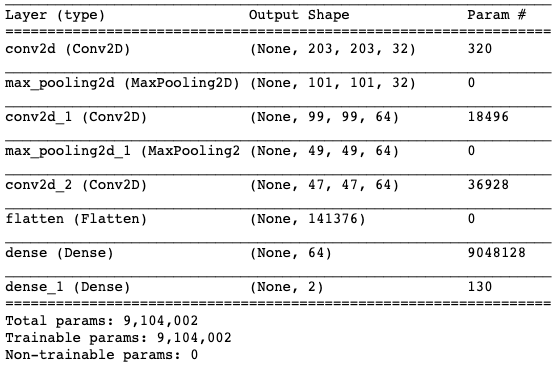
\includegraphics[scale=0.6]{src_img/CNN_pneumonia_archi.png}
    \caption{Architecture de notre modèle de prédiction de pneumonie.}
    \label{CNNPneumoniaArchi}
\end{figure}
Notre modèle prend en argument une image de dimension (205, 205, 1) les deux premières valeurs correspondent à la taille de l'image en pixel et la dernière valeur correspond aux canaux de couleur (1 pour notre cas car l'image est en noir et blanc). L'image vas donc passer dans le premier filtrage (conv2d) qui va nous donner une sortie de dimension (203, 203, 32), nous constatons donc que trente-deux filtres ont été créés sur l'image. Puis ces trente-deux filtres passent par une phase de pooling pour au final avoir une dimension de (101, 101, 32), nous constatons donc que les images ont bien été réduites. On répète l'opération une deuxième fois puis on passe dans la couche "flatten" qui a pour effet de tout représenter sur une liste simple (141 376 correspondant donc à 47 x 47 x 64) afin d'être analysée par une couche de neurones. Cette liste est donc donnée à une couche de soixante-quatre neurones (dense) qui vont l'analyser et passer le résultat à une dernière couche contenant deux neurones (dense\_1) où le résultat d'un neurone correspond à la probabilité que l'image d'entrée montre une pneumonie et l'autre neurone à la probabilité qu'elle n'en montre pas. Ainsi, la convolution nous a fait passer d'une image d'entrée de taille 42 025 (205 x 205, la taille de l'image) à une entrée de taille 141 376. Cela ajoute de la précision à notre modèle, mais a un temps de traitement et de calcul très conséquent. 

\subsection{Explication de notre prédiction}
Notre modèle prêt, nous allons utiliser l'algorithme de LIME présenté dans notre état de l'art afin de vérifier la fiabilité de notre modèle. Dans cette partie, nous n'utiliserons pas la librairie LIME afin de pouvoir entrer plus dans le détail du fonctionnement de cette algorithme et de mieux le comprendre. Le code correspondant à l'implémentions de LIME est disponible sur mon GitHub \cite{limeMyDepot} et suit, entre autre, le tutoriel de "Towards Data Science" \cite{limeTuto}. L'explication sera locale et effectuée sur une seule image. Pour rappel,  l’idée de LIME est de sonder la boite noire autant de fois que nécessaire avec différentes versions de notre image d'entrée qui aura subi de multiples perturbations.\par
La première étape consiste donc à créer des perturbations pour notre image. Pour ce faire, nous allons utiliser la librairie Skimage afin de générer 75 perturbations de notre image. La figure \ref{limePerturbSchema} montre le squelette de perturbation de notre image, chaque zone sera cachée ou affichée comme le montre la figure \ref{limePerturbExemple}.\par
\begin{figure}[h]
    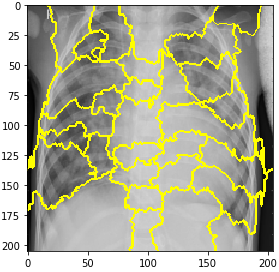
\includegraphics[scale=0.6]{src_img/limePerturbSchema.png}
    \caption{Zones de perturbation}
    \label{limePerturbSchema}
\end{figure}

\begin{figure}[h]
    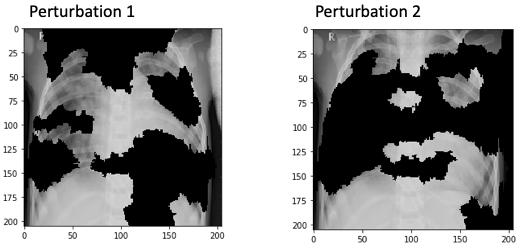
\includegraphics[scale=0.7]{src_img/limePerturbations.png}
    \caption{Exemple de perturbations générées}
    \label{limePerturbExemple}
\end{figure}

La seconde étape consiste à utiliser notre modèle créé précédemment afin d'effectuer une prédiction pour l'ensemble des perturbations générées. La prédiction ne doit pas nous donner le résultat, mais sa probabilité. Pour notre exemple la prédiction ne renverra donc pas "pneumonie", mais un tableau de deux valeurs avec la probabilité d'avoir que les poumons soient sains ou non "[0.23, 0.77]".\par
Une fois nos prédictions faites, nous allons évaluer la distance entre chaque prédiction et notre image de base. La distance correspond aux nombre de zones du squelette de perturbation de la figure \ref{limePerturbSchema} cachées. L'image de base aillant toutes les zones de perturbation visible.\par
Pour finir, nous créons un modèle linéaire que nous entraînons avec les informations obtenues dans les étapes précédentes afin d'obtenir un coefficient pour chacune des zones de perturbations représentant l'importance de la zone pour notre prédiction. Il ne nous reste donc plus qu'à trier ces coefficient afin d'afficher les quatre plus élevés. Pour notre exemple nous obtenons le résultat présenté en figure \ref{limeFinalExplain} sur l'image de gauche.

Afin d'y voir plus clair, nous pouvons superposer l'image obtenue avec l'image de base afin de voir la zone du poumon touchée par la pneumonie selon notre réseau de neurones comme le montre la figure \ref{limeFinalExplain} sur l'image de droite.

\begin{figure}[h]
    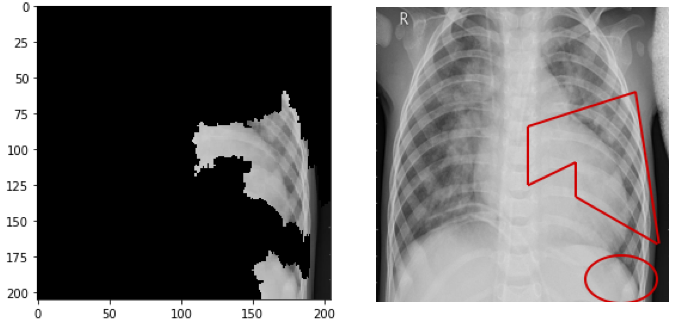
\includegraphics[scale=0.58]{src_img/limeFinalExplainMerge.png}
    \caption{À gauche : Zones de perturbations avec les coefficients les plus élevés
    À droite : Explication de la prédiction de pneumonie par LIME}
    \label{limeFinalExplain}
\end{figure}
\subsection{Bilan}
L'utilisation de l'outil d'interprétabilité nous a donc bien permit de déterminer quelles zones de notre image sont déterminantes pour notre prédiction. Dans notre exemple l'explication apporte un plus à la simple prédiction "pneumonie", car elle montre la zone la plus touchée par la maladie.\par
Accompagner chaque prédiction avec son explication serait un grand plus et améliorer grandement la fiabilité de nos modèles. Aussi, cela permettrai d'augmenter la confiance de la population à l'égard de ces technologies. Bien-sûr le but n'est pas de faire vérifier chaque prédiction par un médecin, cela serai contre-productif et l'IA permettant de faire gagner du temps aux médecins serait inutile. L'idée serait d'utiliser ces prédictions pendant les phases de développement et de test de notre IA afin de vérifier qu'elle évolue dans le bon sens et qu'elle détecte bien les pneumonies et pas autre chose.

\section{Performance}
